%  Template for ICASSP-2021 paper; to be used with:
%          spconf.sty  - ICASSP/ICIP LaTeX style file, and
%          IEEEbib.bst - IEEE bibliography style file.
% --------------------------------------------------------------------------
\documentclass{article}
\usepackage{spconf,amsmath,graphicx}

% Example definitions.
% --------------------
\def\x{{\mathbf x}}
\def\L{{\cal L}}

% Title.
% ------
\title{AUTHOR GUIDELINES FOR ICASSP 2021 PROCEEDINGS MANUSCRIPTS}
%
% Single address.
% ---------------
\name{Author(s) Name(s)\thanks{Thanks to XYZ agency for funding.}}
\address{Author Affiliation(s)}
%
% For example:
% ------------
%\address{School\\
%	Department\\
%	Address}
%
% Two addresses (uncomment and modify for two-address case).
% ----------------------------------------------------------
%\twoauthors
%  {A. Author-one, B. Author-two\sthanks{Thanks to XYZ agency for funding.}}
%	{School A-B\\
%	Department A-B\\
%	Address A-B}
%  {C. Author-three, D. Author-four\sthanks{The fourth author performed the work
%	while at ...}}
%	{School C-D\\
%	Department C-D\\
%	Address C-D}
%
\begin{document}
%\ninept
%
\maketitle
%
\section{Introduction}
\label{sec:intro}

These guidelines include complete descriptions of the fonts, spacing, and
related information for producing your proceedings manuscripts. Please follow
them and if you have any questions, direct them to Conference Management
Services, Inc.: Phone +1-979-846-6800 or email
to \\\texttt{papers@2021.ieeeicassp.org}.

% Below is an example of how to insert images. Delete the ``\vspace'' line,
% uncomment the preceding line ``\centerline...'' and replace ``imageX.ps''
% with a suitable PostScript file name.
% -------------------------------------------------------------------------
\begin{figure}[htb]

  \begin{minipage}[b]{1.0\linewidth}
    \centering
    \centerline{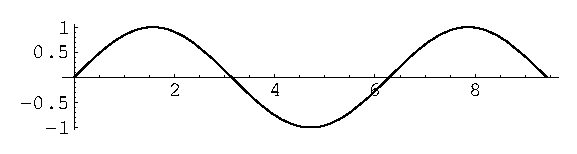
\includegraphics[width=8.5cm]{image1}}
  %  \vspace{2.0cm}
    \centerline{(a) Result 1}\medskip
  \end{minipage}
  %
  \begin{minipage}[b]{.48\linewidth}
    \centering
    \centerline{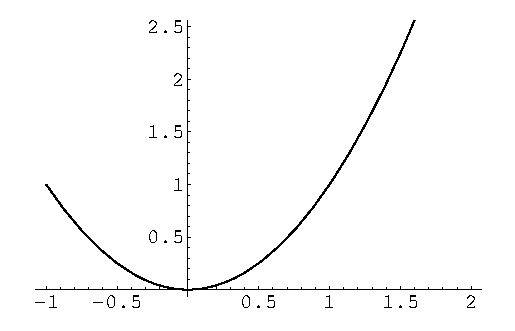
\includegraphics[width=4.0cm]{image3}}
  %  \vspace{1.5cm}
    \centerline{(b) Results 3}\medskip
  \end{minipage}
  \hfill
  \begin{minipage}[b]{0.48\linewidth}
    \centering
    \centerline{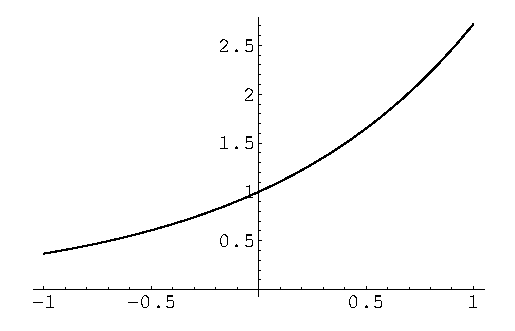
\includegraphics[width=4.0cm]{image4}}
  %  \vspace{1.5cm}
    \centerline{(c) Result 4}\medskip
  \end{minipage}
  %
  \caption{Example of placing a figure with experimental results.}
  \label{fig:res}
  %
  \end{figure}
  

\section{THEORY}
\label{sec:theory}

All printed material, including text, illustrations, and charts, must be kept
within a print area of 7 inches (178 mm) wide by 9 inches (229 mm) high. Do
not write or print anything outside the print area. The top margin must be 1
inch (25 mm), except for the title page, and the left margin must be 0.75 inch
(19 mm).  All {\it text} must be in a two-column format. Columns are to be 3.39
inches (86 mm) wide, with a 0.24 inch (6 mm) space between them. Text must be
fully justified.

\section{RESULTS}
\label{sec:results}

The paper title (on the first page) should begin 1.38 inches (35 mm) from the
top edge of the page, centered, completely capitalized, and in Times 14-point,
boldface type.  The authors' name(s) and affiliation(s) appear below the title
in capital and lower case letters.  Papers with multiple authors and
affiliations may require two or more lines for this information. Please note
that papers should not be submitted blind; include the authors' names on the
PDF.

\section{CONCLUSION}
\label{sec:conclusion}

To achieve {\bf not} the best rendering both in printed proceedings and electronic proceedings, we
strongly encourage you to use Times-Roman font.  In addition, this will give
the proceedings a more uniform look.  Use a font that is no smaller than nine
point type throughout the paper, including figure captions.

In nine point type font, capital letters are 2 mm high.  {\bf If you use the
smallest point size, there should be no more than 3.2 lines/cm (8 lines/inch)
vertically.}  This is a minimum spacing; 2.75 lines/cm (7 lines/inch) will make
the paper much more readable.  Larger type sizes require correspondingly larger
vertical spacing.  Please do not double-space your paper.  TrueType or
Postscript Type 1 fonts are preferred.

The first paragraph in each section should not be indented, but all the
following paragraphs within the section should be indented as these paragraphs
demonstrate.

\section{STATEMENT OF ALL TOOLS USED}
\label{sec:statementofalltoolsused}

Major headings, \cite{Lamp86} for example, "1. Introduction", should appear in all capital
letters, bold face if possible, centered in the column, with one blank line
before, and one blank line after. Use a period (".") after the heading number,
not a colon.

\subsection{Subheadings}
\label{ssec:subhead}

Subheadings should appear in lower case (initial word capitalized) in
boldface.  They should start at the left margin on a separate line.
 
\subsubsection{Sub-subheadings}
\label{sssec:subsubhead}

Sub-subheadings, as in this paragraph, are discouraged. However, if you
must use them, they should appear in lower case (initial word
capitalized) and start at the left margin on a separate line, with paragraph
text beginning on the following line.  They should be in italics.

% To start a new column (but not a new page) and help balance the last-page
% column length use \vfill\pagebreak.
% -------------------------------------------------------------------------
%\vfill
%\pagebreak

\vfill\pagebreak

% References should be produced using the bibtex program from suitable
% BiBTeX files (here: strings, refs, manuals). The IEEEbib.bst bibliography
% style file from IEEE produces unsorted bibliography list.
% -------------------------------------------------------------------------
\bibliographystyle{IEEEbib}
\bibliography{strings,refs}

\end{document}
